\begin{frame}
\frametitle{Model Glass Formers: Poly-disperse Systems}

\begin{columns}
\begin{column}{0.35\textwidth}
\only<3>{
\begin{table}[t]%{0.49\textwidth}%[t]
\begin{tabular}{lcccc}
%\hline\hline
Model   & $m$ & $n$ & $\varepsilon$ & $\tilde{r}_c$  \\ \hline
Poly-(12,0) & 12 & 0 & 0.2  & 1.25 \\
Poly-(12,6) & 12 & 6 &0.2  & 2.5  \\
\multirow{2}{*}{Poly-(18,0)} & 18 & 0 & 0.0 & 1.25  \\
     & 18 & 0 & 0.2 & 1.25 \\
\multirow{2}{*}{Poly-(10,6)} & 10 & 6 & 0.1 & 2.5         \\
     & 10 & 6 & 0.2 & 2.5    
%\hline\hline
\end{tabular}
\centering\caption{List of poly-disperse models studied in this work. For all models, $v_0=1$, $\langle \sigma \rangle = 1$. Density $\rho = 1.01$ and $N=32^2$ particles.}
\end{table}
}
\only<4->{
\begin{figure}[t]
    \centering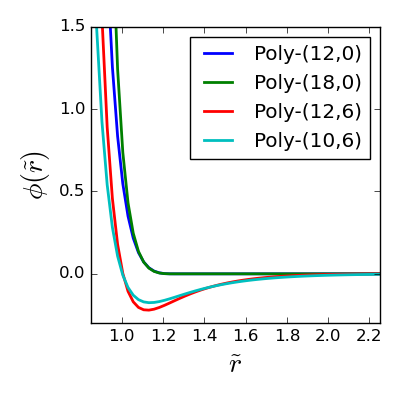
\includegraphics[width=1.1\linewidth]{backup-simulationdetails/pairpotentials.png}
    \caption{Plot of pair potentials for the chosen models.}
\end{figure}

}
\end{column}

\begin{column}{0.65\textwidth}
\only<1->
{
\begin{itemize}
    \item<1-> A class of models given by a power-law particle size distribution $P(\sigma) = A/\sigma^3$ for $\sigma_\mathrm{min} < \sigma < \sigma_\mathrm{max}$ and  pair potential $\phi(r)$ 
    \only<2->
    {
    \begin{align*}
        \phi(r^{\alpha \beta}/\sigma_{\alpha \beta}) =&  v_0\left[\left(\dfrac{\sigma_{\alpha \beta}}{r^{\alpha \beta}}\right)^m-\left(\dfrac{\sigma_{\alpha \beta}}{r^{\alpha \beta}}\right)^n\right] \nonumber
        \\
        & +\sum_{k=0}^{2} c_k \left(\frac{r^{\alpha \beta}}{\sigma_{\alpha \beta}}\right)^{2k} \, \text{for} \  r^{\alpha \beta}/\sigma_{\alpha \beta} \leq \tilde{r}_\mathrm{c}
        \end{align*}
        and $\phi(r^{\alpha \beta}/\sigma_{\alpha \beta})=0$ otherwise where $\sigma_{\alpha \beta}= \frac{1}{2}(\sigma_\alpha+\sigma_\beta)(1-\varepsilon|\sigma_\alpha-\sigma_\beta|)$ and $\varepsilon$ is a non-additivity parameter. 
    }
\end{itemize}
}
\end{column}

\end{columns}

%\begin{column}[T]{0.65\textwidth} and particle size distribution $P(\sigma)$

\end{frame}

\begin{frame}
\frametitle{Simulating Poly-disperse Models}

\begin{columns}
\begin{column}{0.6\textwidth}
\begin{figure}
\begin{overprint}
\onslide<1>\centering\includemedia[height=0.65\textheight,passcontext,transparent,
addresource=backup-simulationdetails/swap_polydisperse.mov,
flashvars={source=backup-simulationdetails/swap_polydisperse.mov}
]{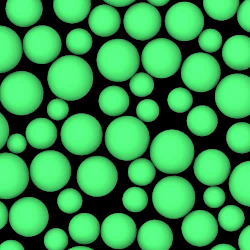
\includegraphics[height=0.65\textheight]{backup-simulationdetails/swap_polydisperse.png}}{VPlayer.swf}
\caption{A swap Monte Carlo simulation using with polydisperse hard disks.} 

\onslide<2>\centering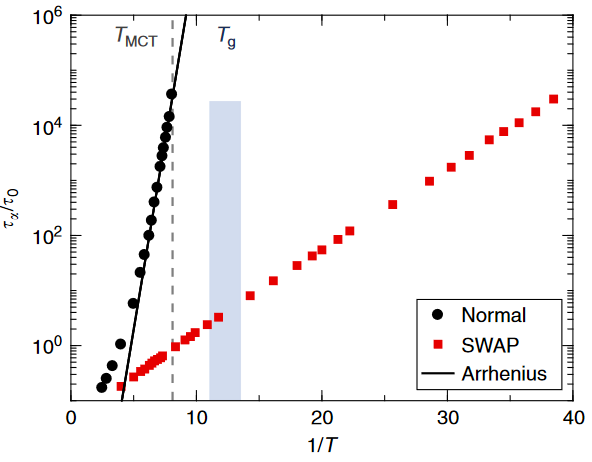
\includegraphics[width=0.80\linewidth]{backup-simulationdetails/poly12_berthier_tau.PNG}\caption{Monte Carlo relaxation time of Poly-(12,0) using translational moves only (Normal) and with swap moves (SWAP), (Berthier, et. al. \textit{Nat. Comm.} 2019). Note the tremendous speed-up in relaxation.}

\onslide<3>\centering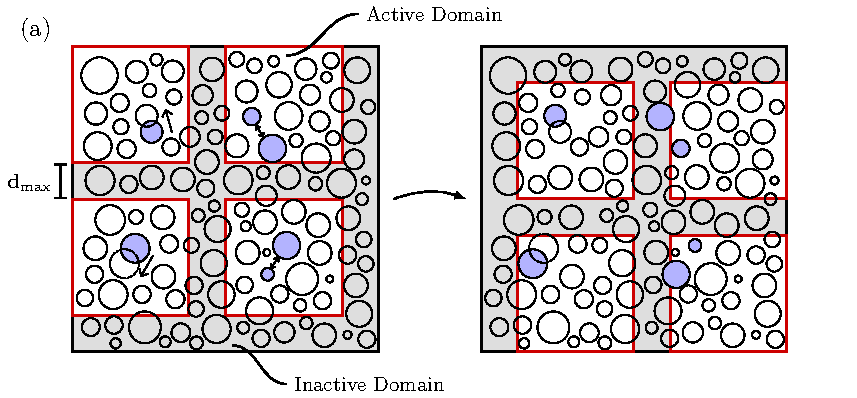
\includegraphics[width=\textwidth]{backup-simulationdetails/ParallelSwapMC_Illustration(3).pdf}\caption{Illustration of parallel swap the parallel version of the swap algorithm, implemented through domain decomposition in HOOMD-Blue.} 

\onslide<4->\centering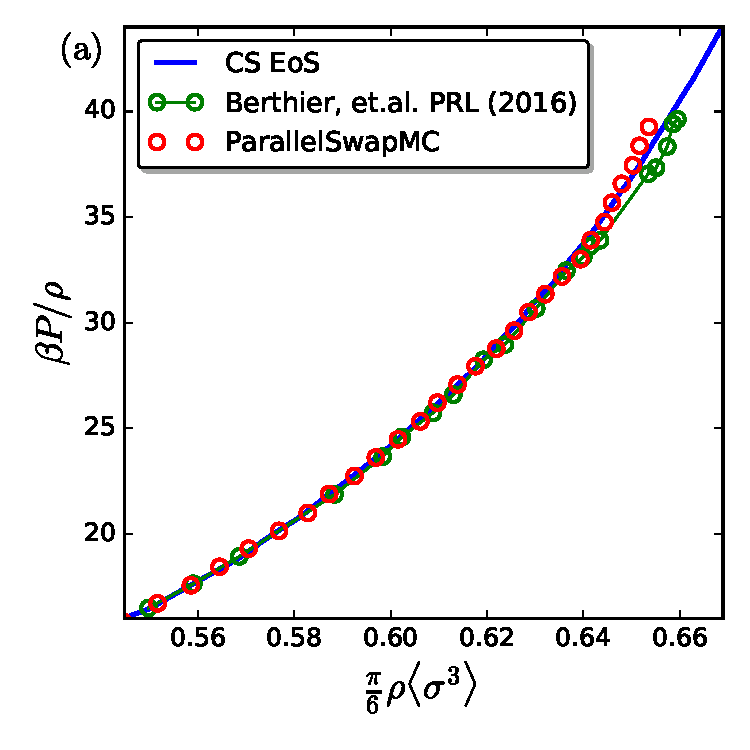
\includegraphics[width=0.48\linewidth]{backup-simulationdetails/3dpolydisperse.pdf}
\centering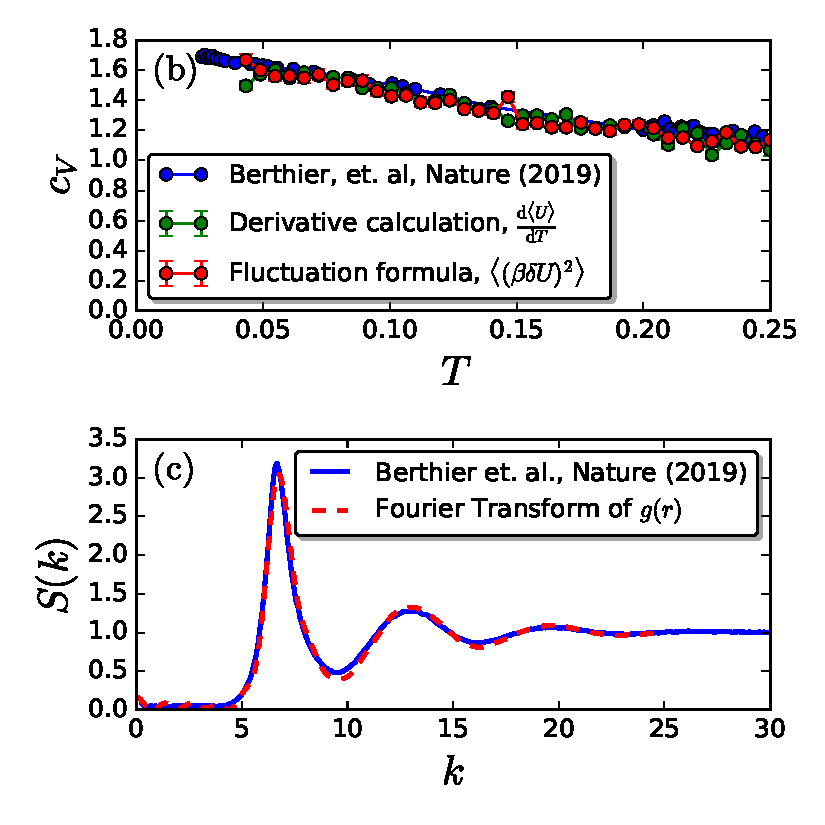
\includegraphics[width=0.48\linewidth]{backup-simulationdetails/2dbenchmark.pdf}
\caption{Parallel swap MC reproduce studies utilizing serial swap MC. (a) EoS of 3D poly-disperse hard spheres (Berthier, et. al. \textit{Phys. Rev. Lett.} 2016), (b) and (c) Heat capacity and structure factor of 2D Poly-(12,0) (Berthier, et. al. \textit{Nat. Comm.} 2019).} 
\end{overprint}

\end{figure}

\end{column}

\begin{column}{0.4\textwidth}
\begin{itemize}
    %\item<2-> The MC swap algorithm allows tremendous speed up in relaxation dynamics and thus, enable studies at ultra-low temperatures.
    \item<1-> All polydisperse models are equilibrated with the Monte Carlo swap algorithm (Ninarello, et. al. \textit{Phys. Rev. X} 2017). 
    \item<2-> Swap MC allows ultra-low-temperature equilibrium studies!
    \item<3-> Implemented in a parallel version (multi-CPU) as a plugin for HOOMD-Blue's hard particle Monte Carlo (HPMC) code\footnotemark %. 
    \item<5-> MD simulations in HOOMD-Blue with pair potentials implemented in a separate package\footnotemark.
    %\item<3-> Equilibrated samples are then equilibrated further in an NVT MD simulation (Nose-Hoover thermostat). Production runs are then done in an NVE simulation. 
    %\item<1-2> At temperatures $T \ll T_\mathrm{o}$, where $T_\mathrm{o}$ is the onset temperature, particles hop. The transition time from its latest position to the next one is called \textit{the instanton time} ß$\Delta t_a$. 
\end{itemize}

\end{column}

\end{columns}

\vspace{-40pt}
\only<3->{\footnotetext{\href{https://github.com/mandadapu-group/parallel-swap-mc}{https://github.com/mandadapu-group/parallel-swap-mc}}}
\only<5->{\footnotetext{\href{https://github.com/mandadapu-group/polydisperse-md}{https://github.com/mandadapu-group/polydisperse-md}}}

\end{frame}

\begin{frame}[c]
\frametitle{Elasticity Tensor and Stress Calculations}
% \only<1-3>
% {
% \begin{itemize}
%     \item<1-> Computing $G^\mathrm{IS}$ requires the computation of a pseudoinverse of the (sparse) Hessian matrix
%     \begin{equation*}
%     \underline{\* H}^+ = \sum_{n=d+1}^{3N} \frac{\underline{\* w}^n \otimes \underline{\* w}^n }{\lambda_n} 
%     \end{equation*}
%     where $\* w^n$ and $\lambda_n$ are the $n$-th eigenvector and eigenvalue.
%     \item<2-> Because we need to do a \textbf{full} eigendecomposition, the computation scales like $O\left((dN)^3\right)$, e.g., Arnoldi iteration to get $dN$ eigenmodes.
%     \item<3-> 
% \end{itemize}
% }

\begin{columns}[c]
\begin{column}{0.5\textwidth}
\begin{figure}
\begin{overprint}
\onslide<2>\centering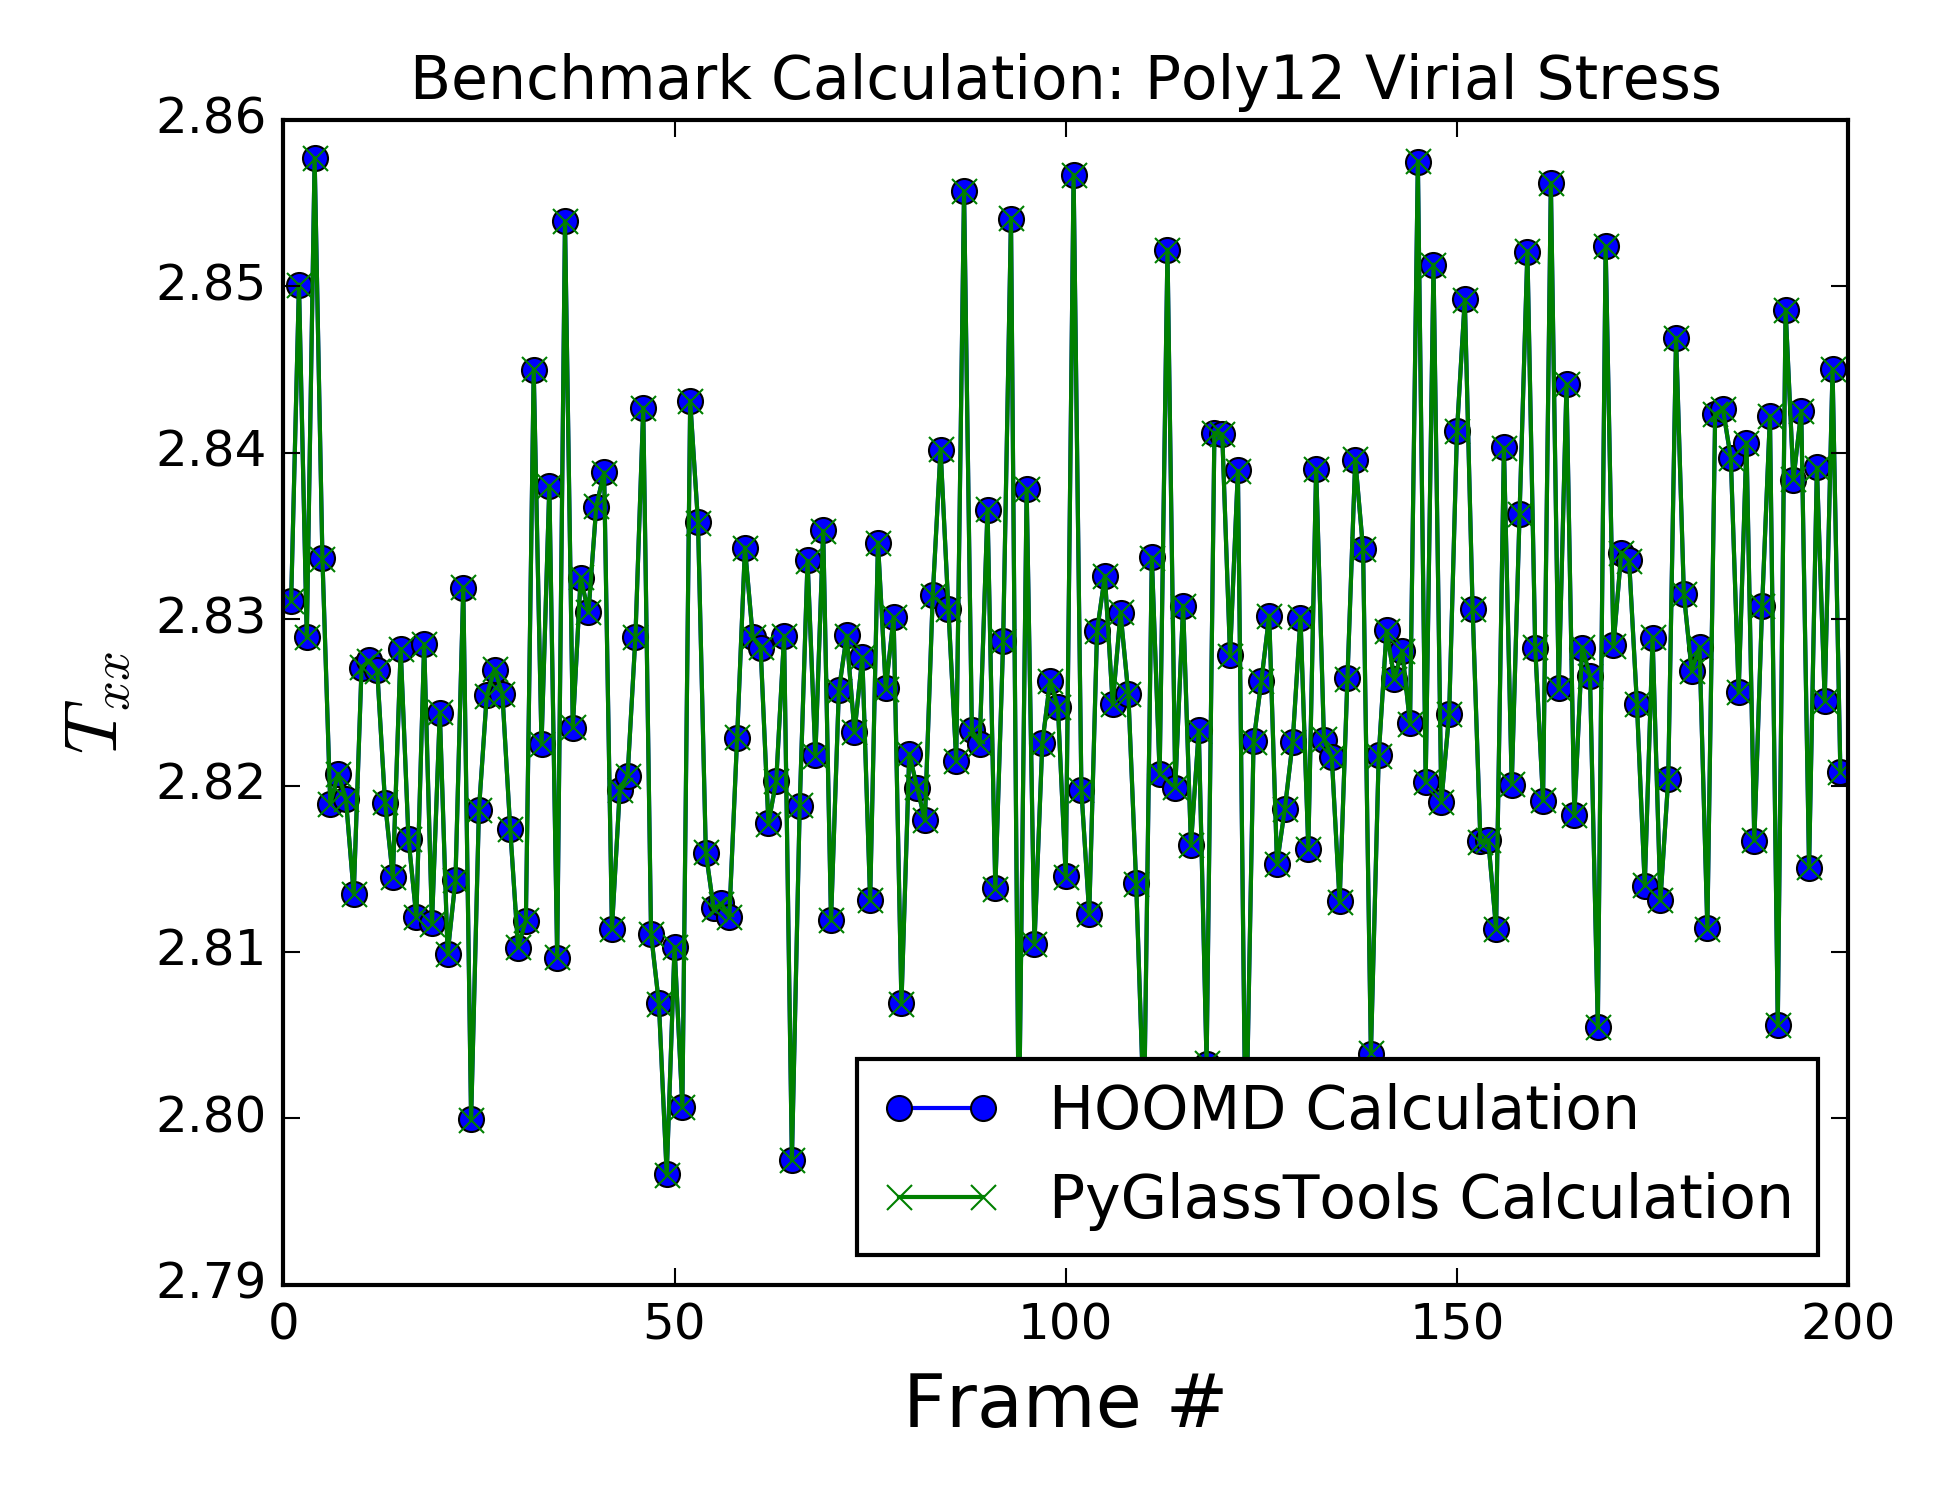
\includegraphics[width=\linewidth]{backup-simulationdetails/benchmarkthermo.png}
    \caption{The package can calculate macroscopic observables that are consistent with other open-source codes.}
\onslide<3>\centering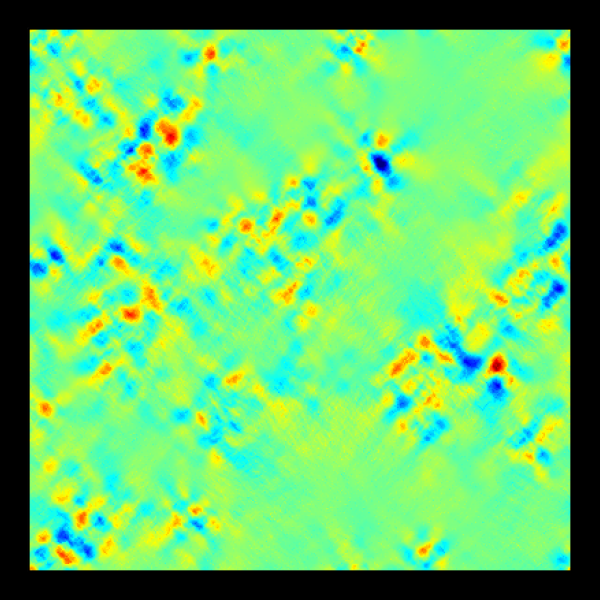
\includegraphics[height=0.7\textheight]{backup-simulationdetails/stresstraj.png}\caption{The change in virial stress $T_\mathrm{xy}(\* x)$ along an inherent-state trajectory.}
\onslide<4>\centering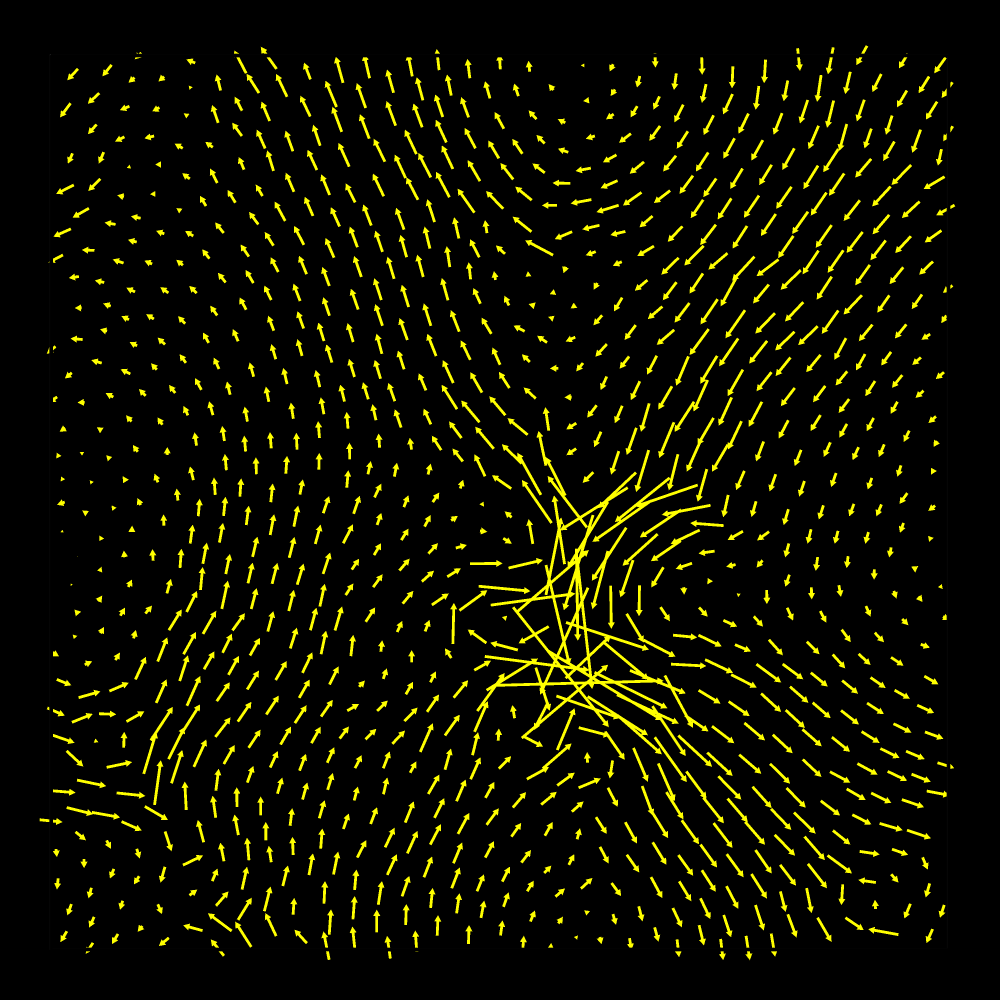
\includegraphics[height=0.7\textheight]{backup-simulationdetails/eigen_small.png}\caption{The lowest eigenmode of a small Poly-(12,0) system ($N=32^2$).}
\onslide<5>\centering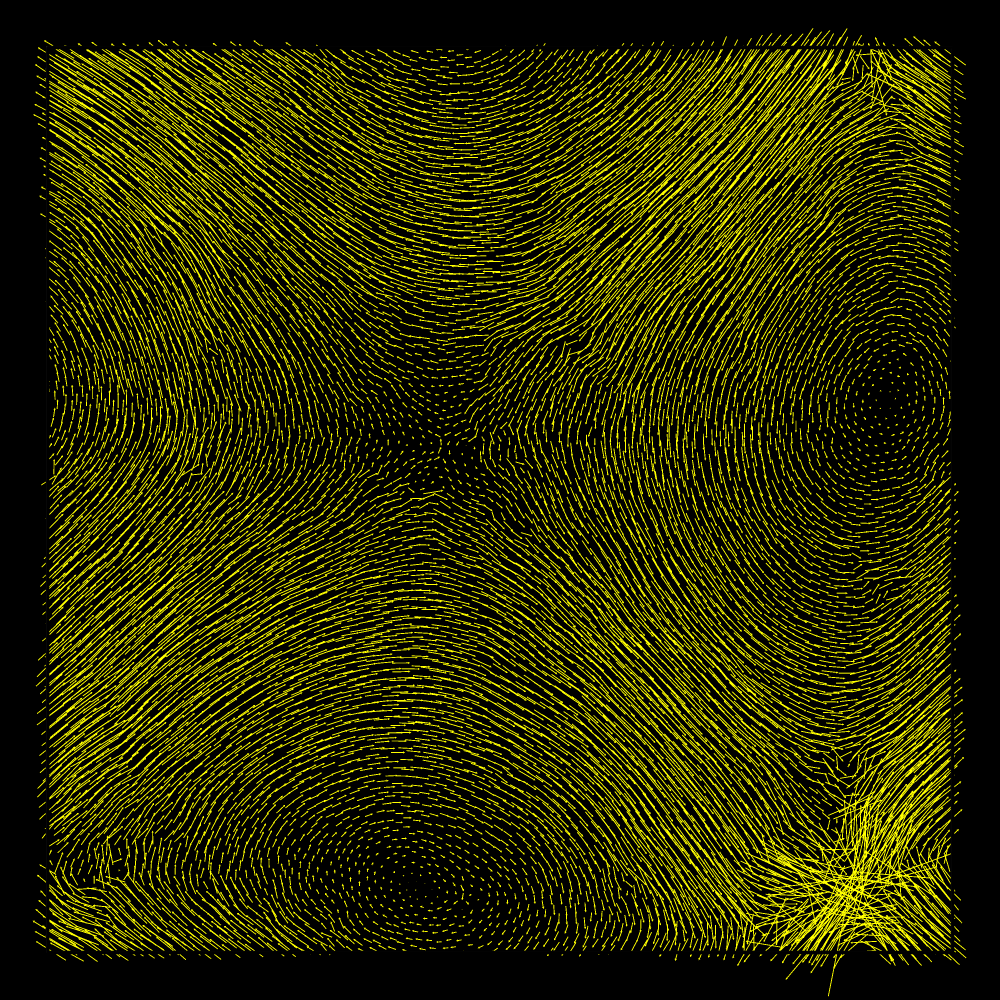
\includegraphics[height=0.7\textheight]{backup-simulationdetails/eigen_large.png}\caption{The lowest eigenmode of a large Poly-(12,0) system ($N=100^2$).}
\onslide<6>\centering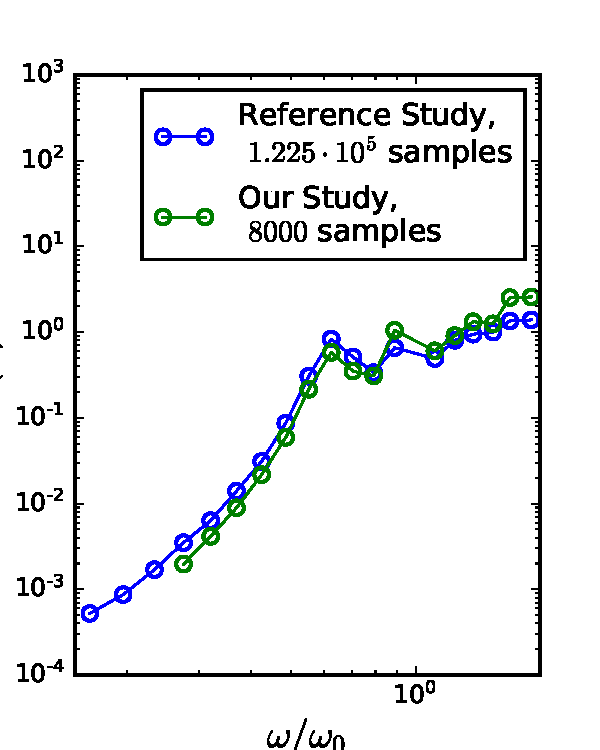
\includegraphics[height=0.7\textheight]{backup-simulationdetails/vdos_lerner.pdf}\caption{The vibrational density of states of a binary soft-disk system. Reference study: (Kapteijns, Bouchbinder, Lerner, \textit{Phys. Rev. Lett.} 2018)}
\end{overprint}
\end{figure}
\end{column} 

\begin{column}{0.5\textwidth}

Developed a Python package \texttt{pyglasstools}\footnotemark to perform parallelized post-processing calculations:
\begin{enumerate}
    \item<2-> \texttt{pyglasstools.thermo}: To compute  virial stress, Born elasticity tensor, and other macroscopic observables. 
    \item<3-> \texttt{pyglasstools.irvingkirkwood}: To compute Irving-Kirkwood fields with arbitrary choice of coarse-graining functions and quadrature methods.
    \item<4-> \texttt{pyglasstools.elasticity}: To perform normal mode analysis and compute non-affine elasticity tensor.
\end{enumerate}

\end{column}

\end{columns}
\only<2->{
\vspace{1em}
\footnotetext{https://github.com/mandadapu-group/pyglasstools}
}
    
\end{frame}